\chapter{Introduction}
First we shall introduce the most important characters in our following exploration. The ideas and definitions here will be recurring regularly as we examine them from different perspectives and using different tools. The content covered by this course can be found in the following books. For further details on some of the results, we recommend consulting these.
\begin{itemize}
	\item J. Guckenheimer \& P. Holmes, Nonlinear Oscillations, Dynamical Systems and Bifurcations of Vector Fields \cite{GuckenheimerHolmes};
	\item F. Verhulst, Nonlinear Differential Equations and Dynamical Systems \cite{Verhulst};
	\item V. I. Arnold, Ordinary Differential Equations \cite{Arnold};
	\item S. Strogatz, Nonlinear Dynamics and Chaos \cite{Strogatz}.
\end{itemize}


\begin{definition}[Dynamical System (DS)]
	A triple $(P,E, \mathcal{F})$, with
	\begin{itemize}
		\item $P :$ the phase space for the dynamical variable ${x} \in P$,
		\item  $E:$ base space of the evolutionary variable (e.g. time) $t \in E$,
		\item $\mathcal{F}: $ the evolution rule (deterministic) which defines the transition from one state to the next.
\end{itemize}
\end{definition}
The two main types of evolutionary variable spaces are
\begin{enumerate}
	\item Discrete dynamical systems (DDS) $t\in E=\mathbb{Z}$ with trajectory $\{ {x}_0,  {x}_1, \ldots\}$,
	\item Continuous dynamical systems (CDS) $t\in E=\mathbb{R}$ with trajectory $\{ {x}_t\}_{t \in \mathbb{R}}$.
\end{enumerate}
Corresponding to these there are various types of evolution rules
\begin{enumerate}
	\item In a DDS we have iterated mappings 
	\begin{align}
		\boxed{ {x}_{n+1} = F( {x}_n , n).}	
	\end{align}
	If there is no explicit dependence on $n$, i.e. $\frac{\partial F}{\partial n} = 0$, then 
	\begin{align}
		\boxed{  {x}_{n+1} F( {x}_n) = F(F( {x}_{n-1})) = \underbrace{F \circ \ldots \circ F}_{n+1 \textrm{ times} }( {x}_0) = F^{n+1}( {x}_0).}
	\end{align}
\begin{ex}[Cobweb diagram of a one-dimensional DDSs]
	In such cases and in one-dimensional problems, a simple way to analyze the behavior of the system is the so-called \textit{cobweb} diagram. We may plot $x_{n+1}$ as a function of $x_{n}$, as demonstrated in Fig. \ref{fig:cobweb}. The image of an initial condition $x_0$ lies on the graph at $x_{n+1}=F(x_0)$. We can also compute the next iterate by horizontally projecting the point $(x_0, F(x_0))$ to the diagonal line defined by $x_{n+1}= x_n$. Following the porjection of this point to the horizontal axis $(x_n)$ we find the intersection with the graph at the point $(x_1, F(x_1))$. It follows that fixed points on the cobweb diagram correspond to the intersection of the graph of $F$ with the diagonal line $x_{n+1}= x_n$.
	\begin{figure}[h!]
	\centering
	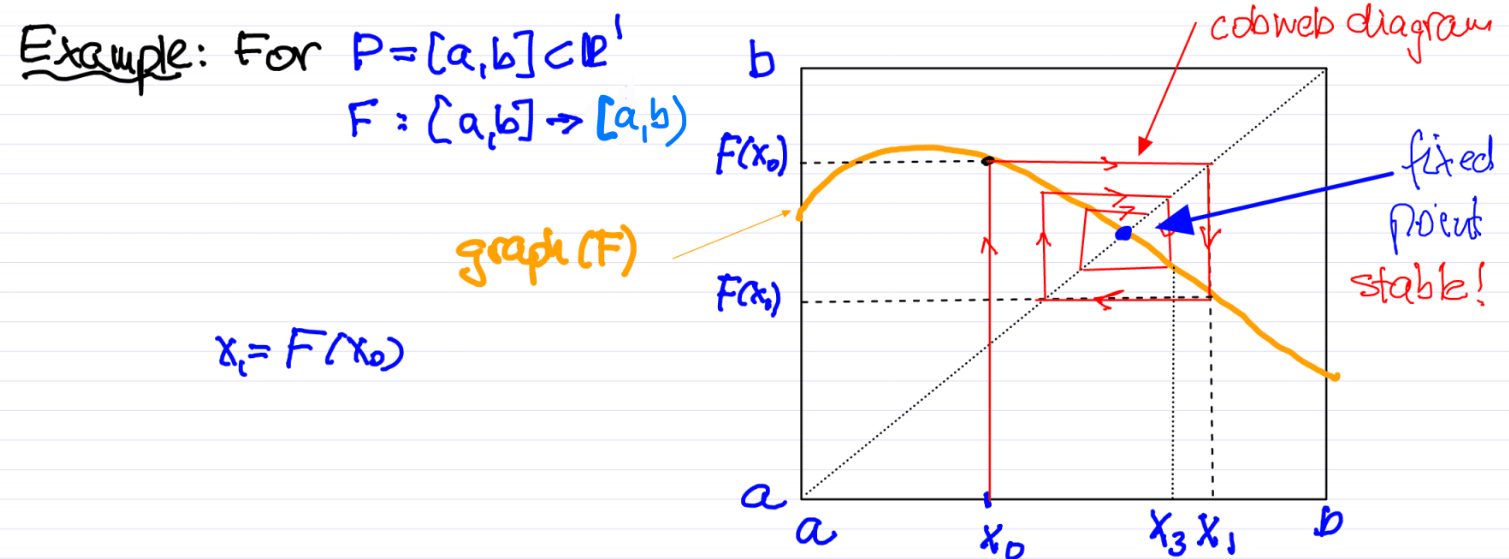
\includegraphics[width = \textwidth]{figures/intro/1DDS.png}
	\caption{Analysis of a one-dimensional system defined on the interval $x\in [a,b]$ using the cobweb diagram} \label{fig:cobweb}
\end{figure}
\end{ex}

\item In a CDS we have a first order system of ordinary differential equations (ODE)
	\begin{align}
		\boxed{
			\dot{ {x}} = f( {x},t)
		}
	\end{align}
	for $ {x}\in P$ and $t \in E$. This yields the initial value problem (IVP):
	\begin{align}
		\begin{dcases}
			\dot{ {x}} = f( {x},t) \\
			 {x}(t_0) =  {x}_0
		\end{dcases}
	\end{align}
	Assuming there exists a unique solution $\varphi(t; t_0,  {x}_0)$ with $\dot{\varphi} = f(\phi,t)$ and $\varphi(t_0)=  {x}_0$, then the following flow map is well defined
	\begin{align}
		\boxed{
		F_{t_0}^{t}( {x}_0) := \varphi(t; t_0,  {x}_0).}
	\end{align}

Geometrically, this solution can be viewed as a trajectory in phase space (cf. Fig. \ref{fig:cds_traj}).
	\begin{figure}[h!]
	\centering
	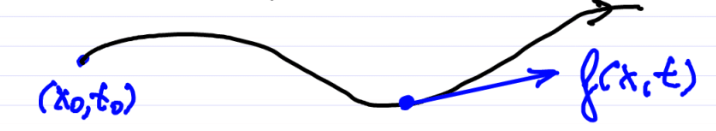
\includegraphics[width = 0.8\textwidth]{figures/intro/2CDS.png}
	\caption{Trajectory of a continuous dynamical system. The RHS is given by f(x,t), which is the tangent vector to this curve at the point $x$ at time $t$.} \label{fig:cds_traj}
	\end{figure}
	
	Such an $F_{t_0}^{t}$ has the properties
	\begin{enumerate}
		\item $F_{t_0}^{t}$ is as smooth as $f( {x},t)$,
		\item $F_{t_0}^{t_0} = I$ and $F_{t_0}^{t_2} = F_{t_1}^{t_2} \circ F_{t_0}^{t_1}$,
		\item $\left(F_{t_0}^{t}\right)^{-1} = F_{t}^{t_0}$ exists and is smooth.
\end{enumerate}
Properties (a) and (b) together are called the group property. A special case of continuous dynamical systems is the autonomous system.
\begin{align}
	\boxed{\dot{ {x}} = f( {x}).}	
\end{align}
The autonomy of a system implies
\begin{align}
	 {x}(s,t_0,  {x}_0) =  {x}(\underbrace{s-t_0}_{t}, 0,  {x}_0) \stackrel{!}{=}  {x}(t, {x}_0).
\end{align}
The induced flow map in this case is the one-parameter family of maps
\begin{align}
	\boxed{ F^{t} = F_{0}^{t}:  {x}_0 \mapsto  {x}(t, {x}_0).}
\end{align}
\end{enumerate}
\begin{ex}[Logisitic Equation]
	For a resource-limited population, we have the following dynamical system for $a> 0$, $b> 0$, and the population $x\in \mathbb{R}_+ \cup \{0\}$
	\begin{align}
		\dot{x} = ax(b-x).
	\end{align}
	In this case we have $E=\mathbb{R}$ and $\mathcal{F} = \{F^{t}\}_{t=-\infty }^{+\infty }$. This system has globally existing unique solutions (see later). We may analyze the behavior of this system by plotting $\dot{x}$ as a function of $x$, analogously to the cobweb diagram. This is demonstrated in Fig. \ref{fig:cds_analysis}. At $x$ values, where $\dot{x}$ is positive $x(t)$ is growing, while at negative values it is decreasing. This means, that fixed points, at which $x(t)=$ const. correspond to intersections of the graphs with the horizontal axis.
	\begin{figure}[h!]
		\centering
		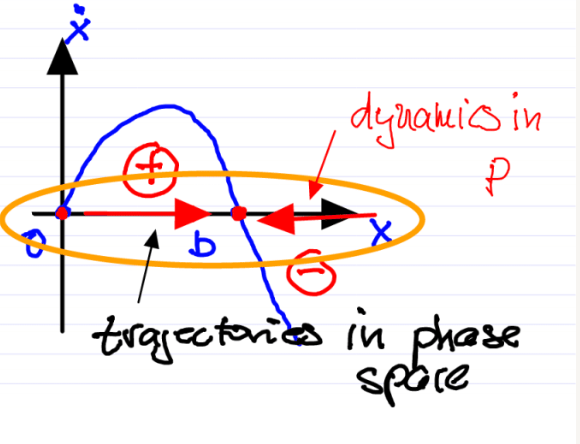
\includegraphics[width=0.4\textwidth]{figures/intro/3RHS.png}	
		\hspace{0.05\textwidth}
		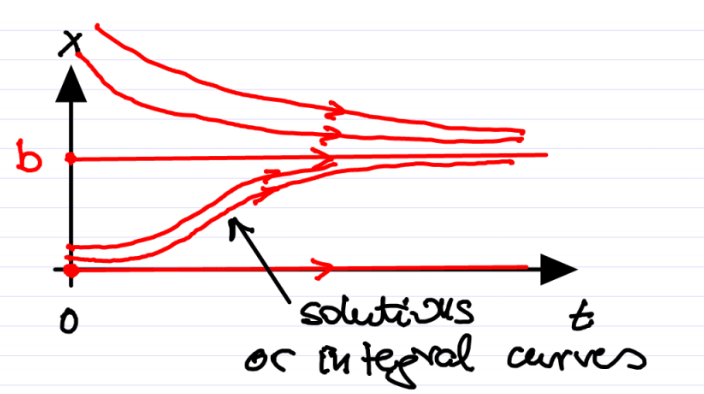
\includegraphics[width=0.4\textwidth]{figures/intro/4solutions.png}
		\caption{Left: Analysis of the right hand side. Right: Evolution in the extended phase space $P \times \mathbb{R}$.} \label{fig:cds_analysis}
	\end{figure}

\end{ex}

\begin{ex}[Pendulum]
Given the equation of motion
\begin{align}
	ml^2 \ddot{\varphi} = -mgl \sin(\varphi).
\end{align}
We let $ x_1 = \varphi$ and $ {x}_2 =\dot{\varphi}$ to transform into the first-order ODE form
\begin{align}
	\begin{dcases}
	\dot{x}_1 = x_2 \\
\dot{x}_2 = - \frac{g}{l} \sin (x_1).
	\end{dcases}
\end{align}
Thus we have 
\begin{align}
 {x} = 
\begin{pmatrix}
	x_1 \\ x_2
\end{pmatrix}; \quad
f( {x}) = 
\begin{pmatrix}
	x_2 \\ - \frac{g}{l}\sin(x_1)	
\end{pmatrix}.
\end{align}
Qualitative analysis gives the following facts
\begin{itemize}
	\item $(x_1, x_2) = (0,0)$ and $(x_1, x_2) = (\pi , 0)$ are zeros of $f$.
	\item Energy is conserved, hence both small and large amplitude oscillations are expected.
	\item The function $f(x)$ has symmetries: it is invariant under the transformation $(x_1, x_2, t) \mapsto (x_1, -x_2, -t)$ and $(x_1, x_2, t) \mapsto (-x_1, x_2, -t)$. See the left panel of Fig. \ref{fig:pendulum_symm+traj}.
\end{itemize}
\begin{figure}[h!]
	\centering
	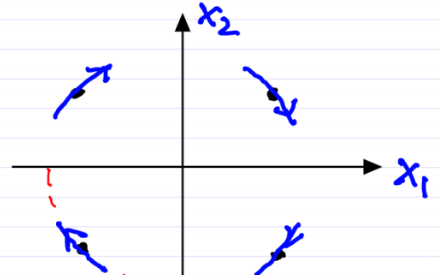
\includegraphics[width=0.4\textwidth]{figures/intro/6pendulum_symmetries.png}
	\hspace{0.05\textwidth}
	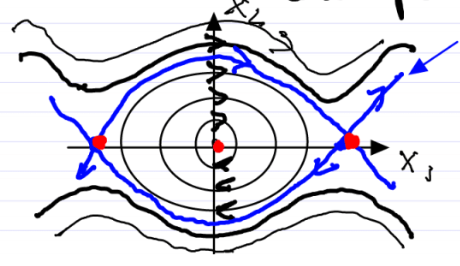
\includegraphics[width=0.4\textwidth]{figures/intro/5pendulum.png}
	\caption{Left: The symmetries of the dynamical system. Right: Phase portrait of the pendulum. Red dots show the fixed points, while the blue trajectories make up the separatrix.} \label{fig:pendulum_symm+traj}
\end{figure}
\begin{definition}
	A separatrix is a boundary (i.e. a codimension-1 surface) in phase space which separates regions of qualitatively different behaviors. In practice, it is unobservable by itself and connects different fixed points. The separatrix of the pendulum is shown in the right panel of Fig. 4.
\end{definition}

\end{ex}

\begin{ex}[Exploit geometry of phase space for analysis]
	Consider two cities, $A$ and $B$. The two cities are connected by two roads, denoted by the blue and green curves of the left panel of Fig. \ref{fig:two_cities}. We assume that travelling on the two roads, it is possible for two bikes to make it from $A$ to $B$ without ever being further away from each other than a distance $d<D$.

Assume two trucks are trying to make it between $A$ and $B$, on different roads in the opposite direction, carrying a load of width $D$. Given this information, can the trucks make it without hitting each other? We can view this problem as a continuous dynamical system with two coordinates $x_1$ and $x_2$ that parameterize the two routes between $A$ and $B$. This dynamical system is, in general, non autonomous.
	\begin{figure}[h!]
		\centering
		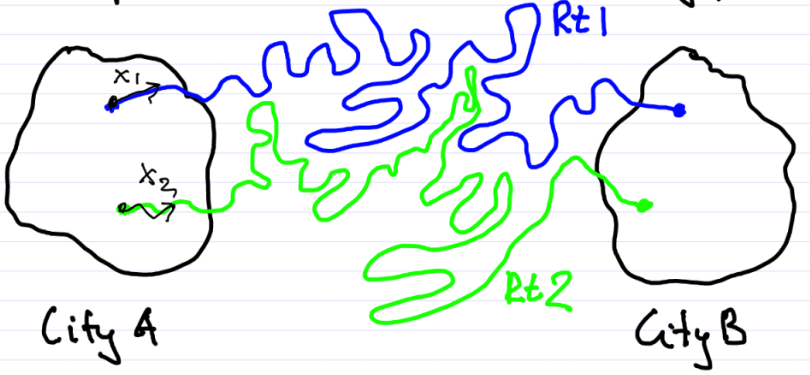
\includegraphics[width=0.5\textwidth]{figures/intro/7routes.png}
		\hspace{0.05\textwidth}
		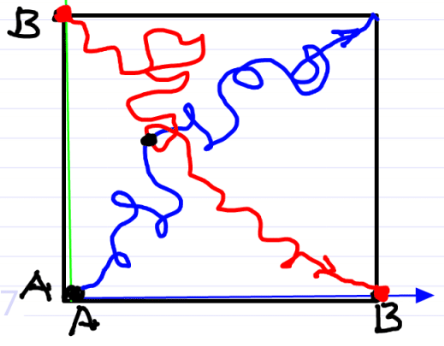
\includegraphics[width=0.3\textwidth]{figures/intro/8truck_geometry.png}
		\caption{Left: An example of the two bike routes. Right: Blue represents the trajectory of the two bikes, red represents the trajectory of the two trucks.} \label{fig:two_cities}
	\end{figure}

	The right panel of Fig \ref{fig:two_cities} shows the trajectories of the two trucks and the two bikes in phase space. The two trajectories must intersect by continuity, thus at that point the trucks must be at the same positions as the bikes, implying they are within distance $D$. Therefore the trucks must crash!	
\end{ex}


